\subsection{Auswertung von falsch erkannten Beziehungen}
\label{subsec:detaillierteAuswertung} 

Im Folgenden sollen die Fälle untersucht werden, in denen der Medextractor falsche Symptom-Krankheit-Zuordnungen findet. Die vom Medextractor analysierten Texte stammen dabei aus drei Quellen:

\begin{enumerate}
	\item Webseite des \emph{National Health Service UK (NHS)} - 49 Texte zu mehreren mentalen Erkrankungen oder Störungen (Agoraphobie, Alkoholmissbrauch, Angststörungen, Essstörungen, Demenz, Depression, Panikstörungen, u.s.w.) \cite{nhs_webpage}
	\item Ein Artikel zum Thema \emph{Mental Disorder} auf Wikipedia \cite{wikimentaldisorder}
	\item Clinical Handbook of Psychological Disorders \cite{clinicalhandbook}
\end{enumerate}

Zur Auswertung dienen die xml-Dateien für den Entity-Linker, da diese auch die Sätze enthalten, in denen Krankheiten bzw. Symptome gefunden wurden. Die Anzahl gefundener Krankheiten, Symptome und Trainingssätze lässt sich einfach durch Zählen der Tags <\textbackslash entity>, <\textbackslash alias> und <\textbackslash sample> ermitteln. Das Ergebnis zeigt Tabelle \ref{tab:zaehlung}. Entitäten bedeuten hierbei Krankheiten und Aliase bedeuten Symptome.

Das in MetaMapLite enthaltene Vokabular erweist sich dabei als umfangreich genug, um zahlreiche richtige Symptom-Krankheit-Relationen zu finden. Man erkennt insbesondere an der Analyse des Handbuchs, dass die Zahl gefundener Begriffe nicht mit dem Umfang des Dokumentes skaliert. Dies liegt (neben der Begrenztheit des Trainingsvokabulars) daran, dass mentale Krankheiten bereits durch die Analyse der kürzeren Texte bereits weitgehend erfasst werden.

Neben den meist richtig erkannten Zusammenhänge finden sich in den xml-Dateien auch einige Zusammenhänge, die vom Medextractor falsch erkannt werden. Häufig liegt dies daran, dass im Trainingsvokabular ungeeignete Begriffe enthalten sind oder dass Grammatik und Semantik eines Satzes unzureichend analysiert werden. Es werden nun in den folgenden Abschnitten typische Fälle untersucht und Wege aufgezeigt, wie insbesondere durch Verwendung der \emph{spaCy}-Pipeline eine Verbesserung des Medextractors erzielt werden könnte.

Da der bisherige Schwerpunkt der Arbeit auf der Verwendung der \emph{Named Entity Recognition} lag und der Standard-NER von \emph{spaCy} in diesem Zusammenhang wenig hilfreich ist, wurden die Stärken von \emph{spaCy} bisher nicht ausgenutzt. Als Ziel sollte verfolgt werden, das Vokabular nicht manuell zu bearbeiten, sondern Algorithmen zu finden, mit denen \emph{spaCy} möglichst automatisch ungeeignete Begriffe erkennt oder auch Begriffe findet, die nicht identisch dem Entity Ruler trainiert wurden.

\begin{table}
\begin{center}
\begin{tabular}{lrrrr}
\hline
\textbf{Quelle}	& \textbf{Dateigröße}	& \textbf{Entitäten} & \textbf{Aliase} & \textbf{Sätze} \\
\hline
NHS &	272 KB & 93 & 221 & 262 \\
Wikipedia & 78 KB & 55 & 67  & 62 \\
Handbook & 3,5 MB & 204 & 485  & 917 \\
\hline
\end{tabular}
\caption{Von Medextractor gefundene Entitäten, Aliase und Beispielsätze}
\label{tab:zaehlung}
\end{center}
\end{table}

\subsubsection{Verben im Symptomvokabular}
\label{subsec: verben} 

Bei Durchsicht der gefundenen Symptom-Krankheit-Relationen fällt zunächst auf, dass das Trainingsvokabular aus MetaMapLite Verben enthält, die zwar bei der Beschreibung von Krankheiten oder Symptomen häufig verwendet werden, für sich allein aber keine Rückschlüsse auf eine Krankheit oder ein Symptom erlauben.

Dazu gehört z.B. das Verb \emph{aggravate}, das auch in den Formen \emph{aggraveted by} und \emph{aggravating} im Vokabular enthalten ist. So wird z.B. in folgendem Satz der Begriff \emph{aggravate} als Symptom einer \emph{anxiety disorder} (Angststörung) gefunden:\\

\emph{\glqq Certain substances such as caffeine ... may aggravate the symptoms of anxiety disorders or interact with prescribed medication.\grqq}\\

Da das Verb \emph{aggravate} allein kein Symptom ist, stellt sich die Frage, wie der Medextractor entscheiden könnte, den hier nun gefundenen Zusammenhang zu verwerfen. Eine Lösung könnte mit Hilfe von \emph{spaCy} erfolgen: der Text lässt sich nämlich auch mit der normale \emph{spaCy}-Pipeline analysieren. Das Ergebnis der grammatikalische Analyse ist in Tabelle \ref{tab:spaCy} wiedergegeben.

\begin{table}
\centering
\begin{tabular}{lllll}
\hline
\textbf{Text}	& \textbf{Lemma}	& \textbf{POS} & \textbf{TAG} & \textbf{DEP} \\
\hline
Certain & certain & ADJ & JJ & amod \\
substances & substance & NOUN & NNS & nsubj \\
such & such & ADJ & JJ & amod \\
as & as & ADP & IN & prep \\
caffeine & caffeine & NOUN & NN & pobj \\
may & may & AUX & MD & aux \\
aggravate & aggravate & VERB & VB & ROOT \\
the & the & DET & DT & det \\
symptoms & symptom & NOUN & NNS & dobj \\
of & of & ADP & IN & prep \\
anxiety & anxiety & NOUN & NN & compound \\
disorders & disorder & NOUN & NNS & pobj \\
or & or & CCONJ & CC & cc \\
interact & interact & VERB & VB & conj \\
with & with & ADP & IN & prep \\
prescribed & prescribed & ADJ & JJ & amod \\
medication & medication & NOUN & NN & pobj \\
\hline
\end{tabular}
\caption{Ergebnis der \emph{spaCy}-Pipeline}
\label{tab:spaCy}
\end{table}

In der Spalte \emph{Text} befinden sich die einzelnen Wörter des zu analysierenden Satzes. Als \emph{Lemma} wird das Grundwort verstanden, also z.B. der Singular (\emph{substance}) eines im Plural stehenden Begriffs (\emph{substances}). 
Das Kürzel \emph{POS} steht für \emph{Part of Speech Tag}. Dies entspricht der Wortart der einzelnen Begriffe. Die grobe Einordnung der Wortarten steht in der Spalte \emph{POS}, während in der Spalte \emph{Tag} eine genauere Bestimmung der Wortart eingetragen ist. Dazu gehört u.a. bei Substantiven die Unterscheidung zwischen Singular und Plural sowie bei Verben die Zeitform.

An dieser Stelle kann bereits festgehalten werden, dass die Wortart des Verbs \emph{aggravate} von \emph{spaCy} richtig erkannt wird. Der Tag \emph{VB} drückt aus, dass das Verb in der Infinitiv-Form vorliegt. In der Spalte \emph{DEP} werden Abhängigkeiten der Wörter untereinander charakterisiert. So wird \emph{aggravate} als zentrales Verb (\emph{root}) des Satzes identifiziert. Mit \emph{nsubj} wird das Subjekt des Satzes markiert, hier also der Begriff \emph{substances}.

Eine Verbesserung des Medextractors könnte nun dadurch erfolgen, dass die Sätze, in denen Symptome und Krankheiten gefunden wurden, zusätzlich durch die \emph{spaCy}-Pipeline analysiert werden und einfache Verben, die sich im Trainingsvokabular befinden, ignoriert werden.

\subsubsection{Generische Überbegriffe}
\label{subsec: generisch} 

Im Trainingsvokabular finden sich generische Überbegriffe wie z.B. \emph{ailments} (Beschwerden, Krankheiten), die ebenfalls weder als konkrete Krankheit oder Symptom taugen. Im folgenden Satz wird \emph{ailments} als Symptom einer \emph{anxiety disorder} gefunden:\\

\emph{\glqq Depression often occurs in children ... experiencing loss, or having ... anxiety disorders and other chronic physical ailments.\grqq}\\

Wie könnte hier nun der Medextractor entscheiden, ob \emph{ailments} ein konkreter oder doch eher ein generischer Begriff ist? Der Dependency-Parser von \emph{spaCy} erkennt, dass in diesem Satz der Begriff \emph{ailments} in einer Konjunktion zum Begriff \emph{disorder} steht und dass das Wort \emph{other} zu \emph{ailments} gehört. Der Medextractor könnte z.B. an dem Wort \emph{other} erkennen, dass der Begriff \emph{ailments} wahrscheinlich eher generischer Natur ist.

\subsubsection{Mehrdeutige Begriffe}
\label{subsec: mehrdeutig} 

Einige Begriffe im Trainingsvokabular sind mehrdeutig und werden daher mitunter irrtümlich als Krankheit oder Symptom gedeutet. Dies ist z.B. für den Begriff \emph{cut} in folgendem Satz der Fall:\\

\emph{\glqq A dependent drinker usually experiences physical and psychological withdrawal symptoms if they suddenly cut down or stop drinking.\grqq}\\

\emph{Withdrawal symptoms} (Entzugserscheinungen) werden daher falsch als Symptom von Schnitt(wunden) erkannt. In diesem Fall kann erneut der Ansatz helfen, keine Verben als Krankheiten zu akzeptieren. Auch wenn \emph{cut} sowohl Nomen als auch Verb sein kann, ist \emph{spaCy} in der Lage, zu erkennen, dass \emph{cut} in diesem Satz ein Verb ist.

Ähnlich verhält es sich mit dem Begriff \emph{cold}. Der Medextractor findet in folgendem Satz fälschlicherweise den Zusammenhang \emph{cold} - \emph {physical signs}:\\

\emph{\glqq You may also notice physical signs and symptoms such as feeling cold, dizzy or very tired.\grqq}\\

Dabei deutet der Medextractor \emph{cold} (Erkältung) als Krankheit und \emph{physical signs} als Symptom.  Durch Analyse mit \emph{spaCy} lässt sich bestimmen, dass \emph{cold} in diesem Satz ein Adjektiv ist, während \emph{spaCy} etwa in dem Satz \emph{\glqq I have a bad cold.\grqq} das Wort \emph{cold} als Nomen identifiziert. Ähnlich wie Verben, sollten einzelne Adjektive nicht als Krankheit gewertet werden.

\subsubsection{Adjektive}
\label{subsec: adjektiv} 

Bei Symptomen können Adjektive nicht ohne weiteres ignoriert werden. Allerdings kommen sie, sofern sie ein Symptom beschreiben, häufig mit einem Verb wie \emph{feeling} vor, also etwa \emph{feeling cold}, \emph{feeling dizzy} oder \emph{feeling very tired}. Tatsächlich enthält das Trainingsvokabular zahlreiche Einträge wie z.B. \emph{feeling angry}, \emph{feeling helpless} oder \emph{feeling bad}. Allerdings fehlen die zuvor genannten und in dem Beispielsatz vorhandenen Ausdrücke.

Es ist daher sinnvoll, alle Adjektive, die mit Verben wie z.B. \emph{feeling} eingeleitet werden, als Symptom zu deuten. Abbildung \ref{fig:dep_parser} zeigt graphisch das Ergebnis der Analyse durch die \emph{spaCy}-Pipeline und zeigt, dass der Dependency Parser einerseits \emph{feeling} und \emph{cold} als zusammengehörig identifiziert (acomp = adjectival complement) und auch erkennt, dass die weiteren Adjektive \emph{dizzy} und \emph{tired} ebenfalls über (grammatikalische) Konjunktionen mit dem Verb \emph{feeling} verbunden sind.

\begin{figure}[h]
    \centering
    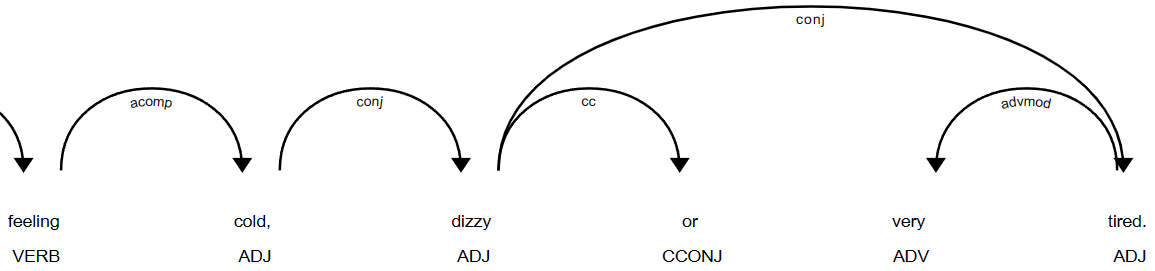
\includegraphics[width=\textwidth]{pictures/Dep_Parser.png}
    \caption{Dependency Parser}
    \label{fig:dep_parser}
\end{figure}

Es eröffnet sich damit eine einfache Methode, auch Symptome, die nicht im Trainingsvokabular enthalten sind, von \emph{spaCy} als Symptome erkennen zu lassen.

\subsubsection{Negationen}
\label{subsec: negations} 

In folgendem Satz wird fälschlich vom Medextractor erkannt, dass Interesse ein Symptom einer Depression ist:\\

\emph{\glqq The psychological symptoms of depression include having no motivation or interest in things.\grqq}\\

Dies liegt daran, dass der Medextractor nicht aus dem Zusammenhang erkennt, dass \emph{interest} in diesem Fall negiert ist, auch wenn das \emph{no} lediglich vor \emph{motivation}\ steht. 

\begin{figure}[h]
    \centering
    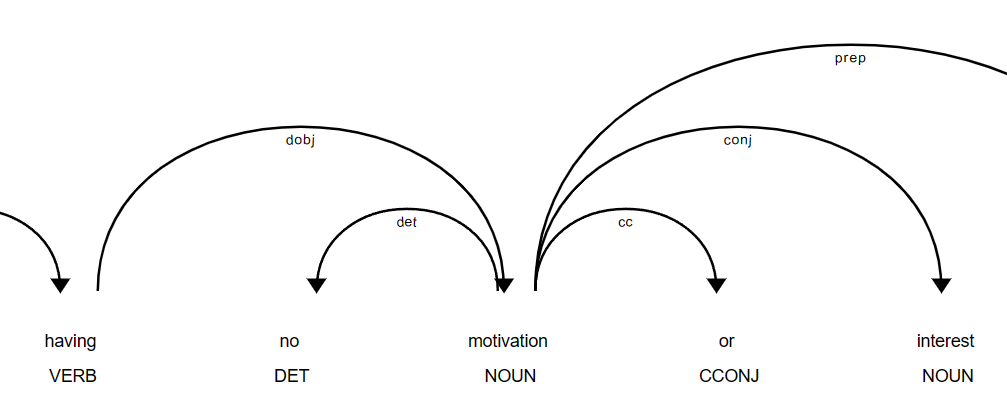
\includegraphics[width=\textwidth]{pictures/Dep_Parser_Negation.png}
    \caption{Dependency Parser bei Negation}
    \label{fig:negation}
\end{figure}

Abbildung \ref{fig:negation} zeigt, dass auch hier der Dependency Parser von \emph{spaCy} gute Dienste leisten kann. Er erkennt, dass \emph{motivation} und \emph{interest} über eine Konjunktion miteinander verbunden sind und dass \emph{no} damit sowohl die Begriffe {motivation} als auch \emph{interest} näher bestimmt.

\subsubsection{Korrelation zwischen Krankheit und Symptom}
\label{subsec: stigmatisierung} 

Kann von einer Krankheit relativ sicher auf Symptome geschlossen werden, so ist der umgekehrte Schluss von Symptom auf Krankheit häufig jedoch sehr unsicher. Ein Beispiel ist der Begriff \emph{anxiety} (Angst / Besorgnis). Bei der Analyse des Handbuchs findet der Medextractor diesen Begriff im Zusammenhang mit über 70 Krankheiten / Störungen. Dieser Umstand ermöglicht es einer Software, automatisch zu erkennen, dass ein Symptom oder Befund keinen sicheren Rückschluss auf eine Krankheit erlaubt. Auch kann durch Auswertung der Häufigkeit ein Modell entwickelt werden, um die Aussagekraft eines Befund zu bewerten.

Problematischer ist es aber z.B. mit dem Zusammenhang \emph{agoraphobia} - \emph{chest pain}, der in dem Satz:\\

\emph{\glqq The physical symptoms of agoraphobia can be similar to those of a panic attack and may include chest pain.\grqq}\\

gefunden wird. Da nur Texte über psychische Erkrankungen untersucht wurden, erscheinen Brustschmerzen nun als eindeutig der Agoraphobie (Angst vor Menschenansammlungen) zugeordnet zu sein. Würde man auch andere medizinische Texte untersuchen, so würde deutlicher werden, dass Brustschmerzen allein keinen deutlichen Hinweis auf eine Agoraphobie geben. Es erscheint daher sinnvoll, den Umfang analysierter Texte auf allgemeine medizinische Texte zu erweitern, auch wenn ein Projekt sich nur auf psychologische Themen beschränkt.

In vielen Fällen kann ein voreiliger Rückschluss von Symptom auf Krankheit auch zu Stigmatisierungen führen. So ist zwar ein dementer Mensch oft alt, alte Menschen dürfen aber nicht pauschal für dement gehalten werden. Da der Begriff \emph{aging} im Symptom-Vokabular enthalten ist, findet der Medextractor in dem Satz:\\

\emph{\glqq But dementia is not a normal part of aging.}\grqq\\

den Zusammenhang \emph{dementia} - \emph{aging}. Ähnlich verhält es sich mit dem Satz:\\

\emph{\glqq ...alcohol misuse can lead to social problems ... such as unemployment ...\grqq},\\

in dem der Zusammenhang \emph{alcohol misuse} - \emph{unemployment} gefunden wird. Auch wenn Alter und (Langzeit-)Arbeitslosigkeit keine unbegründeten Indikatoren für psychische oder mentale Probleme sind, muss darauf geachtet werden, dass eine Software nicht stigmatisierend agiert. Hier kann wahrscheinlich nicht auf ein automatisches Erkennen gesetzt werden, sondern die Software-Entwickler müssen sicherstellen, dass ihre Software mit Begriffen wie Arbeitslosigkeit und Alter angemessen umgeht. Im Fall des Medextractors könnten solche Begriffe z.B. manuell aus dem Vokabular entfernt oder durch Einführung einen Attributes als problematisch markiert werden.

\subsubsection{Bedeutung von Aussagen}
\label{subsec: bedeutung} 

Die einfache Auswertung der gefundenen Entitäten ermöglicht es dem Medextractor nicht, die Bedeutung von Sätzen richtig zu erfassen. In dem Artikel auf Wikipedia findet sich z.B. die Aussage:\\

\emph{\glqq These challenges came ... from gay rights activists who criticised the APA's listing of homosexuality as a mental disorder.\grqq}\\

Hier wird, da auch in dem MetaMapLite Vokabular \emph{homosexuality} als Befund - aber nicht als Krankheit/Störung - enthalten ist, ein Zusammenhang zwischen Homosexualität und einer geistigen Störung gefunden. Dies entspricht aber natürlich nicht der Aussage des Satzes. Um die Bedeutung von Aussagen zu erfassen, ist ein höherer Aufwand zu treiben als in den bisherigen Beispielen. Ein Ansatz könnte sein, in den bisher gefundenen Beispielsätze nach Satzmustern zu suchen, mit denen typischerweise Symptome beschrieben werden. Betrachten wir hierzu den Satz\\

\emph{\glqq Other typical symptoms of severe depression are changes in appetite.\grqq}\\

Hier wird \emph{changes in appetite} als Symptom und \emph{severe depression} als Krankheit gefunden. Dieser Satz beschriebe auch ein Symptom von einer Krankheit, wenn die Begriffe \emph{change of appetite} und \emph{severe depression} durch andere Begriffe aus unserem Vokabular ersetzt würden. Allerdings sind auch viele Abwandlungen dieses Satzes denkbar und es sollte die Zielsetzung verfolgt werden, nach Möglichkeit nicht alle diese Abwandlungen trainieren zu müssen.

\begin{table}
\centering
\begin{tabular}{lllll}
\hline
\textbf{Text}	& \textbf{Lemma}	& \textbf{POS} & \textbf{TAG} & \textbf{DEP} \\
\hline
Other & other & ADJ & JJ & amod \\
typical & typical & ADJ & JJ & amod \\
symptoms & symptom & NOUN & NNS & nsubj \\
of & of & ADP & IN & prep \\
severe & severe & ADJ & JJ & amod \\
depression & depression & NOUN & NN & pobj \\
are & be & AUX & VBP & ROOT \\
changes & change & NOUN & NNS & attr \\
in & in & ADP & IN & prep \\
appetite & appetite & NOUN & NN & pobj \\
.  & . & PUNCT & . & punct \\
\hline
\end{tabular}
\caption{Ergebnis der \emph{spaCy}-Pipeline}
\label{tab:spaCy2}
\end{table}

Mit Hilfe der \emph{spaCy}-Pipeline können Sätze auf ihren Kerninhalt reduziert werden. Dazu wird ein Satz zunächst durch die Pipeline analysiert (s. Tabelle \ref{tab:spaCy2}). In obigem Beispiel wird als zentrales Verb (root) an Position 6 das Wort \emph{are} gefunden. \emph{spaCy} bietet Methoden, mit denen Eltern und Kinder von einzelnen Wörtern gefunden werden können. Die Kinder des Wortes \emph{are} sind z.B. \emph{symptoms} und \emph{changes} (Abbildung \ref{fig:typ_phrase}). 

\begin{figure}[h]
    \centering
    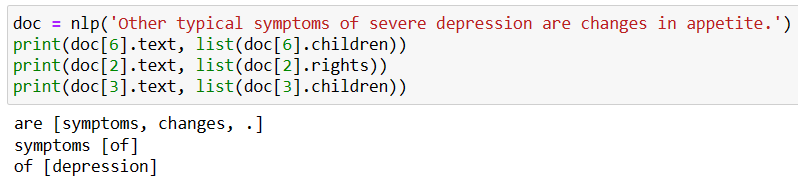
\includegraphics[width=\textwidth]{pictures/Dep_Parser_Text.png}
    \caption{Dependency Parser Ausgabe}
    \label{fig:typ_phrase}
\end{figure}

Man kann nun einen typischen Satz folgendermaßen charakterisieren:

\begin{enumerate}
	\item Die Wurzel (root) des Satzes muss entweder das Verb \emph{is} oder \emph{are} sein.
	\item Eines der Kinder der Wurzel muss als Lemma den Begriff \emph{symptom} besitzen.
	\item Das andere Kind\footnote{Es kann sich auch um mehrere Kinder (also Symptome) handeln.} muss ein Begriff aus dem Symptom-Vokabular sein (ggf. zusammengesetzt).
	\item Rechts neben dem Begriff mit Lemma \emph{Symptoms} steht das Wort \emph{of}.
	\item Das Kind des Begriffs \emph{of} muss ein Begriff aus dem Krankheiten-Vokabular sein (ggf. zusammengesetzt)
\end{enumerate}

Auf diese Weise können auch andere Satzkonstrukte festgelegt werden, mit denen üblicherweise die Symptome von Krankheiten beschrieben werden. Vorteil der bisher sehr einfachen Logik des Medextractors ist, dass alle Beziehungen von Krankheiten und Symptomen in einem Text gefunden werden, sofern die Begriffe im Vokabular enthalten sind. Die vom Medextractor gefundene Sammlung von Beispielsätzen ist daher eine gute Grundlage, um typische Sätze finden zu können.
